\graphicspath{{./images/DBN/}}
\chapter{Extending CPN with Relational Data}
\label{ch:EXT_CPN_RDB}
\paragraph*{\textnormal{This chapter presents an extension of CPN with relational data. An attempt to integrate master data with processes, made by Montali and Rivkin in \cite{DBLP:journals/corr/DBNets}, is presented in this chapter. In this chapter, we will see how coloured petri nets can be extended in order to incorporate relational data. We first give an idea about different layers of DB-nets and how they are interconnected. Later, we will walk through the taxi booking example and modify it to adjust to a DB-net model. Finally, we model the developed DB-net model into CPN Tools. The example for the taxi booking model presented in this chapter is taken from \cite{DBLP:journals/corr/DBNets}.}}

\section{DB-Nets}
\paragraph*{\textnormal{In this section we will build up on the taxi booking example provided in the previous chapter. In this example, the process experts\footnote{process experts are people who are experts on modelling processes.} focus on how the process of booking a taxi is carried out. They may use the petri net model (informally presented in Figure \ref{fig:DBN_PN_Informal}) in order to represent the business process and its requirements, whereas on the other hand the master data experts would take care of requirements about the relevant data of the domain. Then, one can structure the data into classes, provide relationship, constraint etc in order to draft a database schema (informally represented in Figure \ref{fig:DBN_DataModel_Informal}).}}
\begin{figure}[!htbp]
	\centering
	\begin{subfigure}{0.5\textwidth}
		\centering
		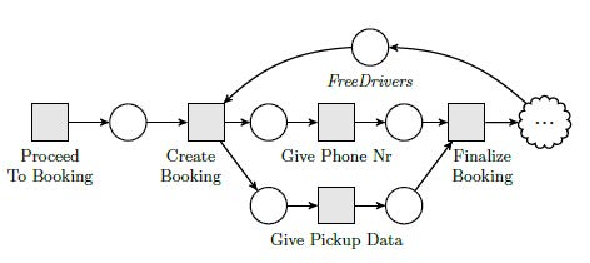
\includegraphics[width=1.0\linewidth]{DBN_PN_Informal.pdf}
		\caption{Process Model}
		\label{fig:DBN_PN_Informal}
	\end{subfigure}%
	\begin{subfigure}{0.5\textwidth}
		\centering
		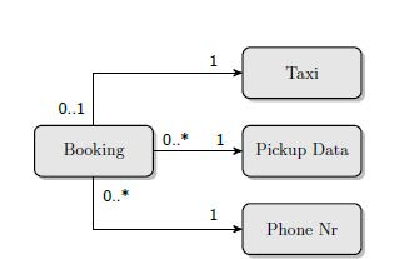
\includegraphics[width=0.7\linewidth]{DBN_DataModel_Informal.pdf}
		\caption{Data Model}
		\label{fig:DBN_DataModel_Informal}
	\end{subfigure}
	\caption{Figure \ref{fig:DBN_PN_Informal} captures the process part informally whereas figure \ref{fig:DBN_DataModel_Informal} captures the data model informally for the taxi booking example.}
	\label{fig:DBN_informal_model}
\end{figure}

\subparagraph*{\textnormal{The problem of integration lies in the example, that in the process flow, while encountering the \textit{Create Booking} transition the process expert would think to create a booking (i.e. instantiate the booking class), whereas from the schema, a booking can only exist in the database only if the corresponding taxi, phone number and the pickup address is provided. With this prospect, during execution one could keep track of free taxi, pickup data and phone number using local variables, and when \textit{Finalize Booking} is called, the corresponding booking entry is created. In this regard, we introduce DB-Nets. In Figure \ref{fig:DBN_Framework}, the framework of the db-nets is presented.}}

\begin{figure}[!htbp]
	\centering
	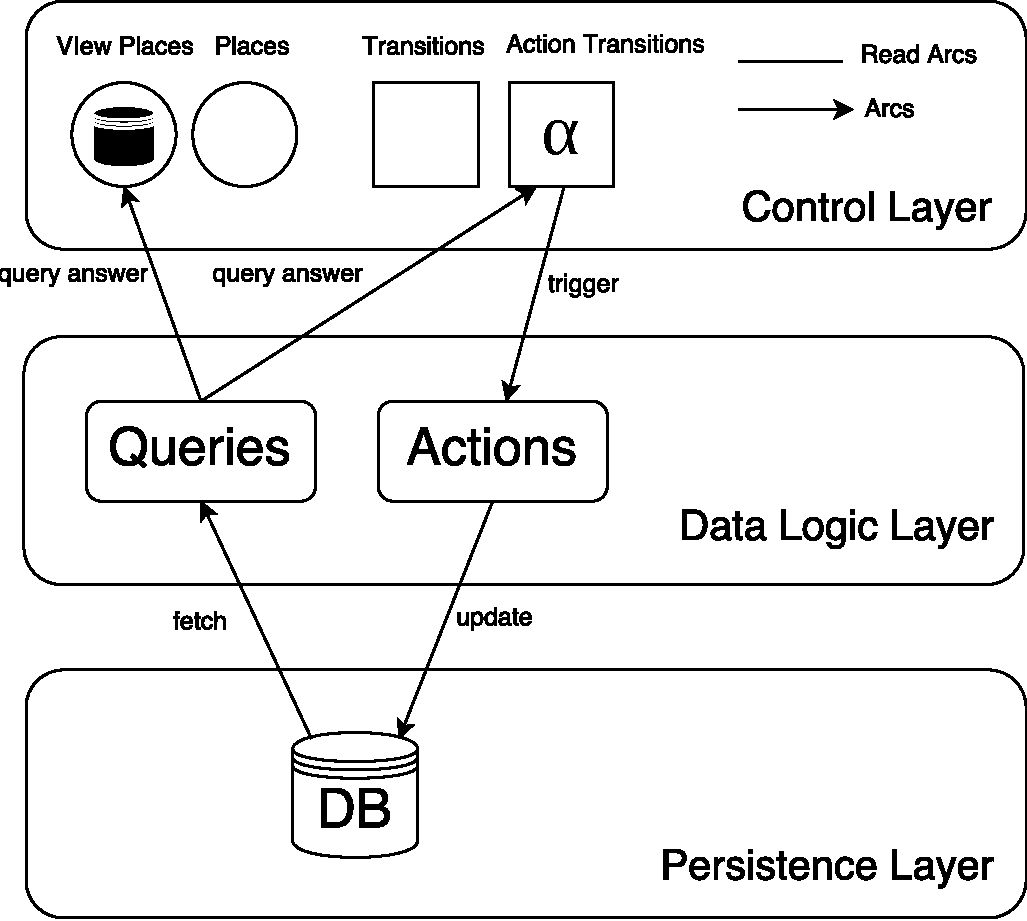
\includegraphics[scale = 0.35]{DBN_Framework.pdf}
	\caption{Framework of the DB-Net model}
	\label{fig:DBN_Framework}
\end{figure}

\subparagraph*{\textnormal{As per \cite{DBLP:journals/corr/DBNets}, the framework comprises of the three layers which are as follows:
		\begin{itemize}
			\item Persistence Layer - contains the full-fledged relational database with constraints. 
			\item Control Layer - process logic is represented with the help of a variant of CPN which supports:
			\begin{enumerate}
				\item typing of tokens, so
				as to account for local variables attached to execution threads.
				\item injection of possibly fresh data values via special so-called $\mathit{\nu}$-variables (leveraging the $\mathit{\nu}$-PN
				model \cite{DBLP:journals/tcs/Rosa-VelardoF11}).
				\item accessing the content of the underlying data layer via special	\textbf{\textit{view-places}}.
				\item updating the underlying data layer by attaching a database update logic to its transitions.
			\end{enumerate} 
			\item Data Logic Layer - used to connect the persistence and the control layer.
		\end{itemize}
}}
\subparagraph*{\textnormal{In figure \ref{fig:DBN_Framework}, the control layer contains a special place called view place, special transitions called action transitions and special arcs called read arcs. The control layer makes use of these special elements to interact with data logic layer in a bidirectional way.}}

\begin{comment}
If we don't intend to consume tokens from a place, then we connect the place with the read arc. The read arc just reads the token value and doesn't remove token from the connected place. The role of rollback arc is to undo the effect of a transition. We would discuss more about this later in the chapter.
\end{comment}

\subparagraph*{\textnormal{The db-net model of the taxi booking example is shown in Figure \ref{fig:DBN_Taxi_Example}. In this example, we assume that from some workflow  \textit{Proceed To Booking} transition is called. Similarly, after the booking is added there may be another workflow. In this example, we are only concerned about the workflow of booking a taxi. Let us see how the three layers (mentioned in the in figure \ref{fig:DBN_Framework}) can be interpreted in the given example (figure \ref{fig:DBN_Taxi_Example}).}}

\begin{figure}[!htbp]
	\centering
	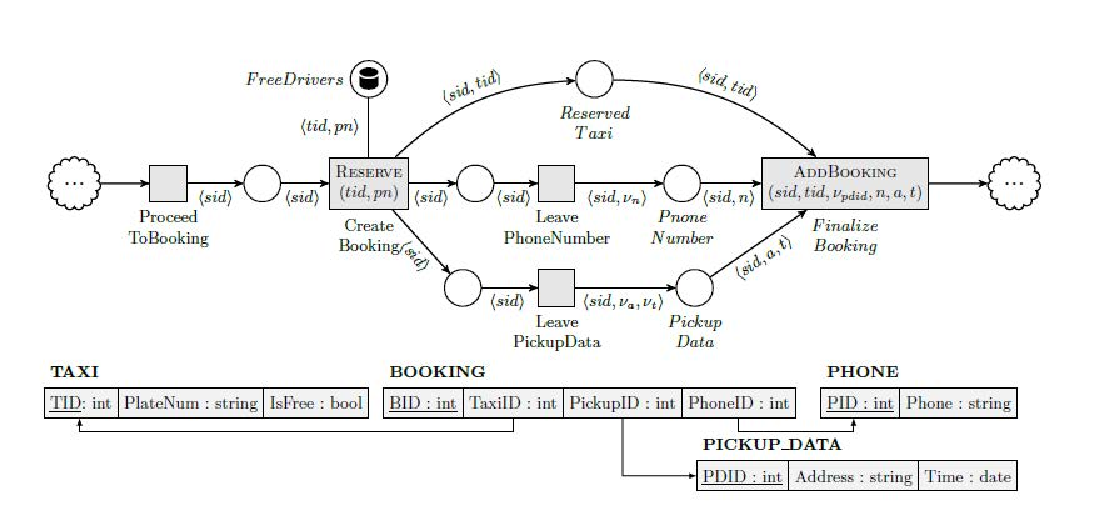
\includegraphics[scale = 0.8]{DBN_Taxi_Example.pdf}
	\caption{A db-net representing the taxi booking process}
	\label{fig:DBN_Taxi_Example}
\end{figure}

\subsubsection{Persistence Layer}
\begin{comment}
\paragraph*{\textnormal{Persistence layer consists of a full-fledged relational databases including constraints. For example, in figure \ref{fig:DBN_Taxi_Example}, the persistence layer consists of the database which contains table \bsq{\textbf{TAXI}}, \bsq{\textbf{BOOKING}}, \bsq{\textbf{PHONE}} and \bsq{\textbf{PICKUP\_DATA}}. The \bsq{TAXI} table consists of 3 columns \bsq{TID} containing integers, \bsq{PlateNum} containing strings and \bsq{IsFree} which contains the boolean value. If a taxi is available then its corresponding record in the \bsq{TAXI} table will have the column $IsFree = \textit{True}$. \bsq{PHONE} table consists of columns \bsq{PID} containing integers and \bsq{Phone} containing the phone numbers as strings. \bsq{PID} is the phone id for a particular phone number. \bsq{PICKUP\_DATA} table contains the pickup data for the customer. The columns in this table are \bsq{PDID} which contains integer, \bsq{Address} containing pickup address as string and \bsq{Time} of type date. \bsq{PDID} is the pickup id for a particular customer's pickup details (address and time). The table \bsq{BOOKING} contains the column \bsq{BID} as integer, \bsq{TaxiID} as integer, \bsq{PickupID} as integer and \bsq{PhoneID} as integer. For a particular record in the \bsq{BOOKING} table, \bsq{BID} denotes the corresponding booking id.}}

\subparagraph*{\textnormal{Along with the table structure, we have also introduced the constraints over it. For example, in the taxi table, a particular \bsq{TAXI} can be uniquely determined from \bsq{TID}. Hence, \bsq{TID} is the primary key (underlined in the figure \ref{fig:DBN_Taxi_Example}). Similarly, each phone number in the \bsq{PHONE} table can be determined by \bsq{PID} and in the table \bsq{PICKUP\_DATA} the pickup details can be determined by \bsq{PDID}. So, these two columns are marked as primary keys. In the \bsq{BOOKING} table, each booking can be determined by \bsq{BID}. \bsq{TaxiID}, \bsq{PickupID} and \bsq{PhoneID} are the foreign keys to the columns \bsq{TID}(in the \bsq{TAXI} table), \bsq{PDID}(in the \bsq{PICKUP\_DATA} table) and \bsq{PID}(in the \bsq{PHONE} table) respectively. This constraints will allow a booking to be added only if it has its corresponding \bsq{TaxiID}, \bsq{PickupID} and \bsq{PhoneID} in the \bsq{TAXI}, \bsq{PICKUP\_DATA} and \bsq{PHONE} table respectively.}}
\end{comment}

\subparagraph*{\textnormal{The persistence layer stores the relevant data for the domain of interest. We consider the relational databases along with its constraints. Using FOL we can express keys, functional dependencies and constraints over the database \cite{BagheriHariri}. For example, in Figure \ref{fig:DBN_Taxi_Example}, different tables are shown along with their functional dependencies and keys. A slight modification in persistence layer is presented in \cite{DBLP:journals/corr/DBNets}.}}

\subparagraph*{\textnormal{As mentioned in the preliminaries (section \ref{sec:preliminaries_relational_db_schema}), we consider the notion of relational schema, sort function and database schema for our need. }}

\begin{comment}
\subparagraph*{\textnormal{We will start with the definition of data type and adopt database schema and relational schema accordingly.}}
\subparagraph*{\textnormal{\todo{here these notions come out of the blue}Inspired from \cite{DBLP:books/aw/found_DB}, we assume \textit{domain} as a countably infinite set $\mathit{\Delta}$, \textit{attributes} as a finite set \textit{\mathit{U}}, and a mapping function $\mathit{dom:U\rightarrow\Delta$ and $dom(A)}$ is called domain of $\mathit{A}$, where $\mathit{A \in U}$.}}

\begin{defs}
\label{defs:dbn_sort_function}
\todo{for all the definitions, please, read carefully page 31 of the cited book. also, try to add more details to your definitions. for example, what does a finitary powerset mean?}
A function \textit{sort} is defined as $sort:R^{n}\rightarrow{\mathcal{P}^{fin}}(U)$, where ${\mathcal{P}^{fin}}$ is the finitary powerset\footnote{the set of finite subsets} of attributes, $R^{n}$ is the set of relation schema and $U$ is the finite set of attributes.
\end{defs}

\subparagraph*{\textnormal{The sort of a relation schema \textit{\mathit{R}} is simply written as $\mathit{sort(R)}$ and the arity is written as $\mathit{arity(R) = |sort(R)|}$. A relational schema ($\mathit{R}$) and set of attributes($\mathit{U}$) together make up the structure of the table. $\mathit{R[U]}$ is used to represent $\mathit{sort(R) = U}$, and $\mathit{R[n]}$ to represent $\mathit{arity(R) = n}$.}}

\begin{defs}
\label{defs:dbn_database_schema}
For a given domain $\Delta$, a \textbf{database schema}\todo{you haven't defined a type function for the database schema} is a non empty finite set $\mathcal{R}$ of relational schemas, written as:
\begin{equation*}
\mathcal{R} = \{R_{1}[U_{1}],\ldots,R_{n}[U_{n}]\}
\end{equation*}
where $R_{1},\ldots,R_{n}$ are relational schemas and $U_{1},\ldots,U_{n}$ are attributes
\end{defs}

\subparagraph*{\textnormal{For example, let \textbf{\textit{taxi\_booking}} be our database schema, shown in Figure \ref{fig:DBN_CPNTools_Taxi_Example}, which is defined by:
\begin{equation*}
\begin{aligned}
\textbf{\textit{taxi\_booking}} =& \{TAXI,\ BOOKING,\ PHONE,\ PICKUP\_DATA\}
\end{aligned}
\end{equation*}
where relational schemas TAXI and PHONE\footnote{One could also write sorts for other relation schemas in the $\textbf{taxi\_booking}$ schema} have the following sorts:
\begin{equation*}
\begin{aligned}
sort(TAXI) = & \{TID,\ PlateNum,\ IsFree\}\\
sort(PHONE)= & \{PID,\ Phone\}
\end{aligned}
\end{equation*}
}}

\subparagraph*{\textnormal{We assume that a \textit{data type} is an infinite set and is defined in a set theoretic manner. For example, \textit{int}, \textit{strings} etc. are \textit{data types}. We define a finite set $\mathit{\Gamma}$ as the set of all data types.}}

\begin{defs}
	\label{defs:dbn_type_function_database}
	A function $\mathit{type_{d}:U \rightarrow \Gamma}$, where $\mathit{U}$ is the set of attributes and $\mathit{\Gamma}$ is the set of data types.
\end{defs}

\subparagraph*{\textnormal{Now we define a typed relational schema as:}}

\begin{defs}
	\label{defs:dbn_typed_relational_schema}
	Given a relation schema $\mathit{R}$ and $\mathit{type_{d}}$ function, a typed relation schema $\mathit{R_{\Delta}}$ is a pair $\mathit{\langle R, type_{d}\rangle}$. 
\end{defs}

\subparagraph*{\textnormal{We extend the notion of the function $\mathit{sort}$, and we define a function $\mathit{sort_{d}}$, such as: }}

\begin{defs}
	\label{defs:dbn_typed_sort_function}
	A function $\mathit{sort_{d}}$ is defined as $\mathit{sort_{d}:R_{\Delta}^{n}\rightarrow{\mathcal{P}^{fin}}(U)}$, where $\mathit{{\mathcal{P}^{fin}}}$ is the finitary powerset\footnote{the set of finite subsets} of attributes, $\mathit{R_{\Delta}^{n}}$ is the set of typed relation schema and $\mathit{U}$ is the finite set of attributes.
\end{defs}

\subparagraph*{\textnormal{The typed sort of a relation schema $\mathit{R_{\Delta}}$ is simply written as $\mathit{sort(R_{\Delta})}$ and the arity is written as $\mathit{arity(R_{\Delta}) = |sort(R_{\Delta})|}$. A typed relational schema ($\mathit{R_{\Delta}}$) and set of attributes($\mathit{U}$) together make up the structure of the table. $\mathit{R_{\Delta}[U]}$ is used to represent $\mathit{sort(R_{\Delta}) = U}$.}}

\begin{defs}
	\label{defs:dbn_typed_database_schema}
	For a given domain $\mathit{\Delta}$, the set of data types $\mathit{\Gamma}$, a \textbf{typed database schema} is a non empty finite set $\mathit{\mathcal{R}_{\Delta}}$ of relational schemas, written as:
	\begin{equation*}
	\mathcal{R}_{\Delta} = \{R_{\Delta_{1}}[U_{1}],\ldots,R_{\Delta_{n}}[U_{n}]\}
	\end{equation*}
	where $\mathit{R_{\Delta_{1}},\ldots,R_{\Delta_{n}}}$ are typed relational schemas and $\mathit{U_{1},\ldots,U_{n}}$ are attributes.
\end{defs}
\end{comment}

\subparagraph*{\textnormal{For example, let \textbf{\textit{taxi\_booking}} be our database schema($\mathcal{R}$), shown in Figure \ref{fig:DBN_Taxi_Example}, which is defined as:
		\begin{equation*}
		\begin{aligned}
		\textbf{\textit{taxi\_booking}} =& \{TAXI,\ BOOKING,\ PHONE,\ PICKUP\_DATA\}
		\end{aligned}
		\end{equation*}
		where relational schemas TAXI and PHONE\footnote{One could also write sorts for other relation schemas in the $\textbf{taxi\_booking}$ schema} have the following sorts and data types:
		\begin{equation*}
		\begin{aligned}
		sort(TAXI) = & \{TID,\ PlateNum,\ IsFree\}\\
		sort(PHONE)= & \{PID,\ Phone\}\\\\
		dom(TID) =\ & int\\
		dom(PlateNum)=\ & string
		\end{aligned}
		\end{equation*}
}}

\begin{defs}
	\label{defs:dbn_rfacts}
	Given a database schema $\mathit{\mathcal{R}}$, a typed relation schema $\mathit{R}$, \textbf{an $\mathit{\mathcal{R}}$ fact} is of the form $\mathit{R(o_{1},\ldots,o_{n})}$ such that $\mathit{o_{i}}$ is an element of a data type and $\mathit{arity(R) = n}$.
\end{defs}

\subparagraph*{\textnormal{Here we will consider a full-fledged typed database schema as our persistence layer.}}
\subsubsection{Data Logic Layer}
\paragraph*{\textnormal{Data Logic Layer is the bidirectional interface between the control layer and the persistence layer. With bidirectional interface, we mean that on one hand we could extract data from an instance of the typed database schema which can be used in the persistence layer where as on the other hand, we could update the instance of the typed database schema by adding and deleting multiple facts at once. If the new database instance obtained after the update is compliant with the persistence layer, the update is committed, otherwise it is rolled back.}}

\subparagraph*{\textnormal{In order to query the database, we use first order logic queries, whereas to update the database instance, we follow the literature on data-centric processes \cite{DBLP:conf/icdt/Vianu09,DBLP:conf/pods/CalvaneseGM13}, where \textit{actions} are used to update database.}}

\begin{defs}
	An \textbf{action} over a persistence layer is a tuple $\mathit{\langle \textbf{n},\vec{p},F^{+},F^{-}\rangle}$, where $\mathit{\textbf{n}}$ is the action name, $\mathit{\vec{p}}$ is a tuple of pairwise distinct typed variables, denoting the \textit{action parameters}, $\mathit{F^{+}}$ and $\mathit{F^{-}}$ respectively represents a finite set of $\mathit{\mathcal{R}_{\Delta}}$-facts over $\mathit{\vec{p}}$, to be added or deleted from the current database instance.
\end{defs}

\subparagraph*{\textnormal{In order to access different components of the action $\mathit{\alpha = \langle \textbf{n},\vec{p},F^{+},F^{-}\rangle}$, we use the dot wise notation: $\mathit{\alpha\cdot}$name = \textbf{n}, $\mathit{\alpha\cdot}$params = $\mathit{\vec{p}}$, $\mathit{\alpha\cdot}$add = $\mathit{F^{+}}$, $\mathit{\alpha\cdot}$del = $\mathit{F^{-}}$. The data logic layer provides a set of actions with which one could update the database instance along with querying the database. For example, on firing the \textit{Create Booking} transition which contains the \textit{RESERVE} action, the database is updated such that the selected taxi is no longer available. The \textit{RESERVE} action has two input parameters, namely \textit{tid} and \textit{pn} denoting taxi id and the plate number respectively. This could be modelled as:
\begin{equation*}
\begin{aligned}
&RESERVE\cdot\textnormal{params} = \langle tid,pn \rangle \\
&RESERVE\cdot\textnormal{del} = \{Taxi(tid,pn,TRUE)\} \\
&RESERVE\cdot\textnormal{add} = \{Taxi(tid,pn,FALSE)\} \\
\end{aligned}
\end{equation*}
The set of FOL queries attached with the actions helps us querying the database and obtain the result. For example, the transition $\mathit{Finalize\ Booking}$, adds a booking to the table \textit{BOOKING} with a unique booking id, which is obtained as an answer to the attached query.}}

\subparagraph*{\textnormal{The data logic layer captures the flow of information from the control layer and performs actions on it. Similarly, this layer is also responsible for receiving the answer to the query from the persistence layer and passing on to the control layer.}}

\subparagraph*{\textnormal{Note that in control layer, we modify the definition of colour-sets ($\mathit{\Sigma}$) and say that colour-sets ($\mathit{\Sigma}$) is the finite set of possibly infinite colour-set. This is intentionally done to make the colour-sets compatible with answers of the queries.}}

\subsubsection{Control Layer}
\paragraph*{\textnormal{ In Figure \ref{fig:DBN_Framework}, the control layer has few additional components, namely, \textit{View places}, \textit{Action Transitions} and \textit{Read arcs}. These components are also incorporated in Figure \ref{fig:DBN_Taxi_Example}. The place $\mathit{Free\ Drivers}$ is a \textit{view place} which shows the currently available taxis. Since the records of the free taxi are stored in the database, they are fetched as an answer on querying the database. The set of view places is represented by $\mathit{P_{v}}$.}}

\begin{defs}
	\label{defs:dbn_query_function}
	A function $\mathit{query_{v}}$ is defined as $\mathit{query_{v} : P_{v} \rightarrow Q}$ where $\mathit{Q}$ is the set of first order logic queries.
\end{defs}

\begin{defs}
	\label{defs:dbn_formal_view_place}
	The set of \textbf{view places} ($\mathit{P_{v}}$) is a set such that:
	\begin{enumerate}
		\item $\mathit{P_{v} \subseteq P}$.
		\item for each $\mathit{p_{v} \in P_{v}}$, $\mathit{query_{v}(p_{v}) = q}$ where $\mathit{q \in Q}$.
		\item the answer $\mathit{(a_{1},\ldots,a_{k})}$ to the query $\mathit{q}$ having free variables $\mathit{(x_{1},\ldots,x_{k})}$, for all $\mathit{p_{v} \in P_{v}}$, $\mathit{(a_{1},\ldots,a_{k}) \in C(p_{v})}$.
		\item Let $\mathit{Ans = \{A_{1}, \ldots,A_{n}\}}$ be the set of answers returned for the query $\mathit{q}$ attached to the view place $\mathit{p_{v}}$, $\mathit{I(p_{v}) = {_{}^{++}\sum\limits_{A \in Ans}^{} {1}^{\backprime}A}}$.
	\end{enumerate}
\end{defs}

\subparagraph*{\textnormal{For example, $P_{v} = \{Free \ Drivers\}$ and for $p_{v} = Free \ Drivers$ we can attach a query to the view place as $query_{v} = Taxi(x,y,\textnormal{TRUE})$. Let us assume that there are two free taxis. The set of answers to the query \[Ans = \{(47552,\textnormal{\bdsq{BR-03NA-5422}}), (49209,\textnormal{\bdsq{BR-01AP-4392})}\}\]. The initialization function for the view place will be:
\begin{equation*}
\begin{aligned}
I(Free\ Drivers) =&\ 1^{\backprime} (47552,\textnormal{\bdsq{BR-03NA-5422}})\\
 &+\!\!+ 1^{\backprime} \textnormal{(49209,\bdsq{BR-01AP-4392}})
\end{aligned}
\end{equation*}
}}

\begin{comment}
\subparagraph*{\textnormal{For example, in order to show the available taxi one could show it by using the following query :}}

\begin{verbatim}
SELECT TID, PlateNum FROM TaxiBooking.TAXI WHERE IsFree = TRUE;
\end{verbatim}

\subparagraph*{\textnormal{In the SQL query above, TaxiBooking.TAXI represents the TAXI table of the schema TaxiBooking. So, it selects the taxi id(TID) and Plate Number(PlateNum), from the table TAXI which is the part of TaxiBooking schema, which is available ($\mathit{IsFree = True}$). Also, the query returns TID and PlateNum hence the colour-set of the view place should be compatible to the return type of the query. In this case the colour-set of the view place can be defined as:}}

\begin{verbatim}
COLSET TAXI = product INT * STRING;
\end{verbatim}

\begin{defs}
\label{defs:view_place}
A \textbf{view place} ($p_{v}$) extends the notion of a normal place in the CPN model. The extension is based on the following aspects:
\begin{enumerate}
\item A view place carry a database query with itself. The attached query should always be a SELECT clause.
\item The colour-set assigned to the view place should match with the data tuple resulted on answering the attached query.
\item View places are not immutable. It can change if the data in the data in the database changes.
\item View places should always be connected with read arcs.
\end{enumerate}
\end{defs}

\subparagraph*{\textnormal{We could formalize the notion of read arcs and view places.}}
\begin{defs}
\label{defs:read_arc}
A \textbf{read arc} extends the notion of a normal arc in the CPN model. The extension is based on the following aspects:
\begin{enumerate}
\item A read arc connects a transition and a view place.
\item In contrast to the normal arcs, the read arcs do not consume tokens from the view places. However, the free variables over the arcs are allowed to get assigned corresponding to an enabled binding if it exists.
\end{enumerate}
\end{defs}
\end{comment}

\subparagraph*{\textnormal{In Figure \ref{fig:DBN_Taxi_Example}, the view place is connected to the $\mathit{Create\ Booking}$ transition through a read arc. In contrast to a normal arc, instead of consuming tokens from the place, the read arc reads the token available at the view place. In the example, the inscription on read arc is $\mathit{\langle tid, pn \rangle}$. Similar to the normal arc, for an enabled binding element, the variables can take part in the assignment. The set of read arcs is represented by $\mathit{A_{r}}$.}}

\begin{defs}
	\label{defs:dbn_formal_read_arc}
	The set of \textbf{read arcs} $\mathit{A_{r}}$, where $\mathit{A_{r} \subseteq (P_{v} \times T) \cup (T \times P_{v})}$ such that:
	\begin{enumerate}
		\item $\mathit{A_{r} \subseteq A}$.
		\item $\mathit{A_{r}}$ is symmetric. i.e. $\mathit{(p_{v},t) \in A_{r}}$ iff $\mathit{(t,p_{v}) \in A_{r}}$ and $\mathit{E((p_{v},t)) = E((t,p_{v}))}$.
		\item For $\mathit{p_{v} \in P_{v}}$ and $\mathit{t \in T}$, $\mathit{(p_{v},t) \not\in (A\setminus A_r)}$ and $\mathit{(t,p_{v}) \not\in (A\setminus A_r)}$.
	\end{enumerate}
\end{defs}
\subparagraph*{\textnormal{The second condition in the Definition \ref{defs:dbn_formal_read_arc} states that, the read arcs cannot consume tokens whereas the third condition restricts \textit{view places} to connect with normal arcs. In the example (see Figure \ref{fig:DBN_Taxi_Example}), the set of read arcs is represented by :
		\begin{equation*}
		A_{r} = \{(Free \ Drivers, Create Booking),(Create Booking, Free \ Drivers) \}
		\end{equation*}}}

\subparagraph*{\textnormal{Along with carrying execution in CPN, the role of transitions in DB-nets are mainly:
		\begin{enumerate}
			\item acquire data from the environment using fresh variables.
			\item perform queries and updates on the persistence layer.
\end{enumerate}}}

\begin{defs}
	For a transition $\mathit{t \in T}$, the set of \textbf{output variables} $\mathit{Var_{out}[t]}$ is the set of variables such that for all pair $\mathit{(t,p) \in A}$, $\mathit{Var_{out}[t] = Var[E((t,p))]}$ where $\mathit{p \in P}$ and $\mathit{E}$ is the expression function.
\end{defs}

\begin{defs}
	For a transition $\mathit{t \in T}$, the set of \textbf{input variables} $\mathit{Var_{in}[t]}$ is the set of variables such that for all pair $\mathit{(p,t) \in A}$, $\mathit{Var_{in}[t] = Var[E((p,t)))]}$ where $\mathit{p \in P}$ and $\mathit{E}$ is the expression function.
\end{defs}

\begin{defs}
	For a transition $\mathit{t \in T}$, the set of \textbf{fresh variables} $\mathit{Var_{f}[t]}$ $\mathit{= Var_{out} \setminus Var_{in}}$.
\end{defs}

\subparagraph*{\textnormal{Note that the outgoing arc of \textit{LEAVE PHONE NUMBER} transition contains an additional variable $v_{n}$. The set of \textit{output variables}, \textit{input variables} and \textit{fresh variables} for \textit{LEAVE PHONE NUMBER} transition is:
\begin{equation*}
\begin{aligned}
&Var_{out}[t] = \{s\_id,v_{n} \} \\
&Var_{in}[t] = \{s\_id\} \\
&Var_{f}[t] = Var_{out}[t] \setminus Var_{in}[t] = \{v_{n}\}
\end{aligned}
\end{equation*}
%In order to avoid modelling complexities, we assume that the $\mathit{\mathcal{R}_\Delta}$ facts to be deleted in $\mathit{F^{-}}$ do not depend on fresh variables. 
Transitions are responsible for performing updates over the database. For example, the transition $\mathit{Create\ Booking}$ reserves the available taxi, and thus updates the database instance by making the selected taxi unavailable for further booking. We call these transitions as \textit{Action Transition}.}}

\begin{defs}
	\label{defs:DBN_transition_action_function}
	A function $\mathit{trans_{act}}$ is a function $\mathit{trans_{act} : T \rightarrow \Lambda}$ where $\mathit{T}$ is the set of transitions and $\mathit{\Lambda}$ is the set of actions.
\end{defs}
\begin{defs}
	\label{defs:dbn_formal_action_transition}
	The set of \textbf{action transitions} $\mathit{T_{a}}$ is a set such that:
	\begin{enumerate}
		\item $\mathit{T_{a} \subseteq T}$.
		\item for all $\mathit{t_{a} \in T_{a}}$, $\mathit{trans_{act}(t_{a})}$ is non-empty.
	\end{enumerate}
\end{defs}

\paragraph*{\textnormal{In the example shown, the set of \textit{action transitions} is given by:
\begin{equation*}
T_{a} = \{Proceed\ To\ Booking, Create\ Booking, Leave\ Phone\ Number, ...\}
\end{equation*}
The fresh variables are used for acquiring data from the external environment. Using all the definitions above we can now formalize the notion of a DB-Net(DBN).}}
\begin{defs}
	\label{defs:DBN_formal_definition_DBN}
	A non-hierarchical DBN is a fifteen-tuple\\{$\mathit{DBN = (P,P_{v},T,T_{a},A,A_{r},\Sigma,V,C,G,E,I,\mathcal{R}_{\Delta},query_{v},trans_{act})}$}, where:
	\begin{itemize}
		\item $\mathit{P,T,A,V,C,G,E,I}$ stands same as defined in CPN.
		\item $\mathit{\Sigma}$ is the finite set of possibly infinite colour-sets.
		\item $\mathit{P_{v}}$ is the set of view places such that $\mathit{P_{v} \subseteq P}$ and a first order logic query assigned to it.
		\item $\mathit{T_{a}}$ is the set of action transitions such that $\mathit{T_{a} \subseteq T}$, which contains actions required to query and update the database.
		\item $\mathit{A_{r}}$ is the set of read arcs such that $\mathit{A_{r} \subseteq A}$, which connects a view place to a transition.
		\item $\mathit{\mathcal{R}_{\Delta}}$ is the full fledged typed database schema.
		\item $\mathit{query_{v}}$, defined as $\mathit{query_{v} : P_{v} \rightarrow Q}$, where $\mathit{Q}$ is the set of FOL queries.
		\item $\mathit{trans_{act}}$, defined as $\mathit{trans_{act}: T \rightarrow \Lambda}$ is a function from the set of transitions to the set of actions.
	\end{itemize}
\end{defs}

\section{DB-Nets Modelling}
\paragraph*{\textnormal{In this section, we will see how to model a DB-Net using CPN Tools in an abstract manner. The DB-Net modelled in CPN Tools\footnote{To know how to use actions in transitions in CPN Tools \cite{CPN_Tools_CodeSegment}.} is shown in Figure \ref{fig:DBN_CPNTools_Taxi_Example}. In CPN Tools, read arcs are not provided. Therefore, instead of read arcs we use double headed arcs, which allow the consumption and regeneration of tokens at the place in a unit time. In this model the set of \textit{view places}, \textit{action transitions} and \textit{read arcs} is given by:
\begin{equation*}
	\begin{aligned}
		P_{v} =& \{Free \ Drivers\}\\
		T_{a} =& \{Create\ Booking, Leave\ Phone\ Number, Leave\ Pickup\ Data,\\
		& Finalize\ Booking\}\\
		A_{r} =& \{(Free \ Drivers, Create Booking),(Create Booking, Free \ Drivers) \}
	\end{aligned}
\end{equation*}
The query attached with the view place is given by:
\begin{equation*}
	query_{v}(Free\ Taxi) = Taxi(TID,PlateNum,TRUE)
\end{equation*}
where \textit{TID} and \textit{PlateNum} are the free variables in the query determining the corresponding taxi id and plate number of the available taxi. The variables of interest for the actions attached to the transitions are taken as parameter in the input clause. Fresh variables are specified in the output clause. For example, in the \textit{Finalize Booking} transition, the variables in the input clause are:
\begin{equation*}
	\{t\_id, v\_n, v\_a, v\_t\}
\end{equation*}
and the fresh variables (for booking id, pickup id and phone id) mentioned in the output clause are:
\begin{equation*}
	\{b\_id,pd\_id,ph\_id\}
\end{equation*}
In the action part, the fresh variables acquire their data from the external environment (e.g. getBookingID()). The \textit{INSERTPHONE} action adds a new entry in the table \textit{PHONE} with the corresponding phone number and the phone id. Note that, \textit{INSERTPHONE} action is followed by \textit{INSERTPICKUP} and \textit{INSERTBOOKING} action to obey the foreign key constraints. Similarly, in the \textit{Create Booking} transition, the \textit{RESERVE} action updates the database instance by making the selected taxi unavailable for further booking.}}

\begin{figure}[!htbp]
	\centering
	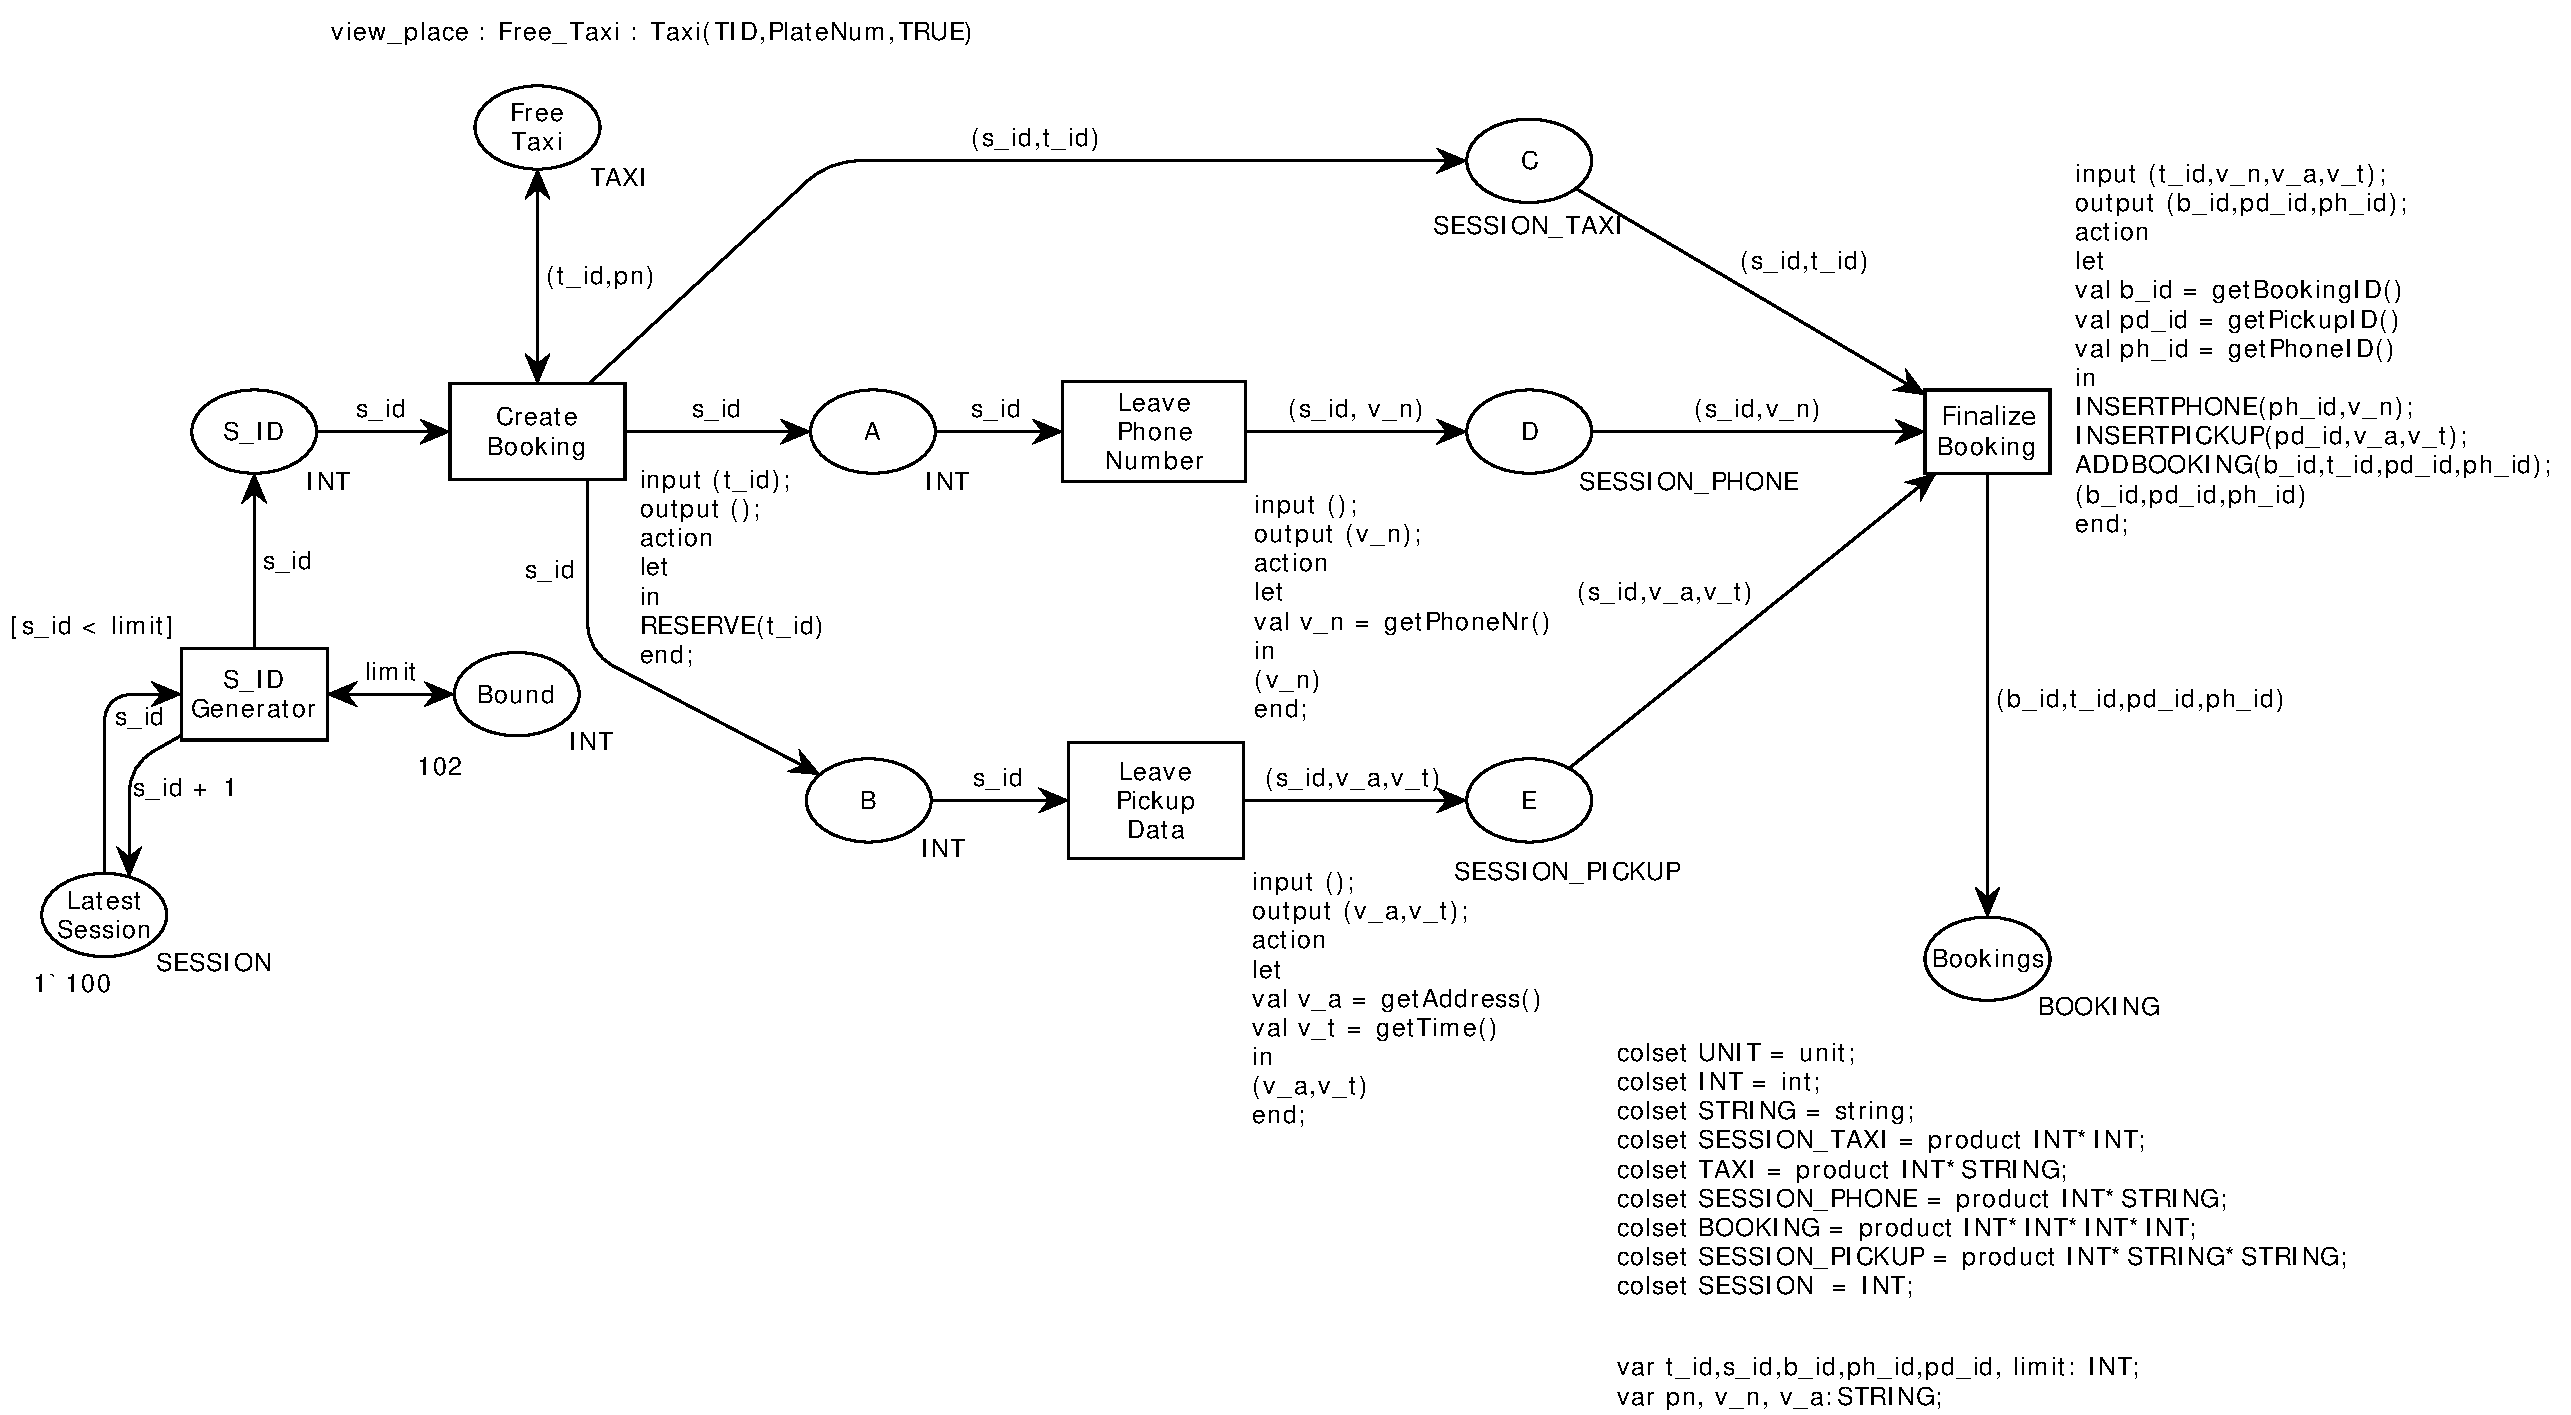
\includegraphics[scale = 0.33]{DBN_CPNTools_Taxi_Example.pdf}
	\caption{A db-net representing the taxi booking process modelled in CPN Tools}
	\label{fig:DBN_CPNTools_Taxi_Example}
\end{figure}

\subparagraph*{\textnormal{The major components in the DB-Nets are view places, read arcs, action transitions, the data logic layer and the data acquisition for fresh variables. Using these we could interact with the persistence layer. The execution semantics of CPNs can be applied over DBN. Additionally, after occurrence of every step, the view places need to be refreshed, e.g. the view place $\mathit{Free\ Taxi}$ needs to be updated when a step occurs in the net.}}

\subparagraph*{\textnormal{In the later chapters, we will see the development and working of the DB-Nets extension for CPN Tools.}}


